
%% ai-pedia-paper.tex
%% AI-Pedia project paper — structure follows L3 CS Project Paper Template (LaTeX)
%% Template: project-paper-template.tex (v1.1, Dec 2022, Craig Stewart)
%% for Durham University, Computer Science Project paper templates
%% contact craig.d.stewart at durham.ac.uk for support
%%
%% Based on IEEE Template: bare_jrnl_compsoc.tex, V1.4b, by Michael Shell
%%
%% Notice from original IEEE Template:
%%*************************************************************************
%% Legal Notice:
%% This code is offered as-is without any warranty either expressed or
%% implied; without even the implied warranty of MERCHANTABILITY or
%% FITNESS FOR A PARTICULAR PURPOSE! 
%% User assumes all risk.
%% In no event shall the IEEE or any contributor to this code be liable for
%% any damages or losses, including, but not limited to, incidental,
%% consequential, or any other damages, resulting from the use or misuse
%% of any information contained here.
%%
%% All comments are the opinions of their respective authors and are not
%% necessarily endorsed by the IEEE.
%%
%% This work is distributed under the LaTeX Project Public License (LPPL)
%% ( http://www.latex-project.org/ ) version 1.3, and may be freely used,
%% distributed and modified. A copy of the LPPL, version 1.3, is included
%% in the base LaTeX documentation of all distributions of LaTeX released
%% 2003/12/01 or later.
%% Retain all contribution notices and credits.
%% ** Modified files should be clearly indicated as such, including  **
%% ** renaming them and changing author support contact information. **
%%*************************************************************************


\documentclass[10pt,journal,compsoc]{IEEEtran}

% Some very useful LaTeX packages include:
% (uncomment the ones you want to load)


%% ---------------------------------------------- START OF USEFUL PACKAGES ----------------------------------------------

%\usepackage{ifpdf}
% Heiko Oberdiek's ifpdf.sty is very useful if you need conditional
% compilation based on whether the output is pdf or dvi.
% usage:
% \ifpdf
%   % pdf code
% \else
%   % dvi code
% \fi
% The latest version of ifpdf.sty can be obtained from:
% http://www.ctan.org/pkg/ifpdf
% Also, note that IEEEtran.cls V1.7 and later provides a builtin
% \ifCLASSINFOpdf conditional that works the same way.
% When switching from latex to pdflatex and vice-versa, the compiler may
% have to be run twice to clear warning/error messages.


% *** CITATION PACKAGES ***
%
\ifCLASSOPTIONcompsoc
  % IEEE Computer Society needs nocompress option
  % requires cite.sty v4.0 or later (November 2003)
  \usepackage[nocompress]{cite}
\else
  % normal IEEE
  \usepackage{cite}
\fi
% cite.sty was written by Donald Arseneau
% V1.6 and later of IEEEtran pre-defines the format of the cite.sty package
% \cite{} output to follow that of the IEEE. Loading the cite package will
% result in citation numbers being automatically sorted and properly
% "compressed/ranged". e.g., [1], [9], [2], [7], [5], [6] without using
% cite.sty will become [1], [2], [5]--[7], [9] using cite.sty. cite.sty's
% \cite will automatically add leading space, if needed. Use cite.sty's
% noadjust option (cite.sty V3.8 and later) if you want to turn this off
% such as if a citation ever needs to be enclosed in parenthesis.
% cite.sty is already installed on most LaTeX systems. Be sure and use
% version 5.0 (2009-03-20) and later if using hyperref.sty.
% The latest version can be obtained at:
% http://www.ctan.org/pkg/cite
% The documentation is contained in the cite.sty file itself.
%
% Note that some packages require special options to format as the Computer
% Society requires. In particular, Computer Society  papers do not use
% compressed citation ranges as is done in typical IEEE papers
% (e.g., [1]-[4]). Instead, they list every citation separately in order
% (e.g., [1], [2], [3], [4]). To get the latter we need to load the cite
% package with the nocompress option which is supported by cite.sty v4.0
% and later. Note also the use of a CLASSOPTION conditional provided by
% IEEEtran.cls V1.7 and later.


% *** GRAPHICS RELATED PACKAGES ***
%
\ifCLASSINFOpdf
  \usepackage[pdftex]{graphicx}
  % declare the path(s) where your graphic files are
  % \graphicspath{{../pdf/}{../jpeg/}}
  % and their extensions so you won't have to specify these with
  % every instance of \includegraphics
  % \DeclareGraphicsExtensions{.pdf,.jpeg,.png}
\else
  % or other class option (dvipsone, dvipdf, if not using dvips). graphicx
  % will default to the driver specified in the system graphics.cfg if no
  % driver is specified.
  % \usepackage[dvips]{graphicx}
  % declare the path(s) where your graphic files are
  % \graphicspath{{../eps/}}
  % and their extensions so you won't have to specify these with
  % every instance of \includegraphics
  % \DeclareGraphicsExtensions{.eps}
\fi
% graphicx was written by David Carlisle and Sebastian Rahtz. It is
% required if you want graphics, photos, etc. graphicx.sty is already
% installed on most LaTeX systems. The latest version and documentation
% can be obtained at: 
% http://www.ctan.org/pkg/graphicx
% Another good source of documentation is "Using Imported Graphics in
% LaTeX2e" by Keith Reckdahl which can be found at:
% http://www.ctan.org/pkg/epslatex
%
% latex, and pdflatex in dvi mode, support graphics in encapsulated
% postscript (.eps) format. pdflatex in pdf mode supports graphics
% in .pdf, .jpeg, .png and .mps (metapost) formats. Users should ensure
% that all non-photo figures use a vector format (.eps, .pdf, .mps) and
% not a bitmapped formats (.jpeg, .png). The IEEE frowns on bitmapped formats
% which can result in "jaggedy"/blurry rendering of lines and letters as
% well as large increases in file sizes.
%
% You can find documentation about the pdfTeX application at:
% http://www.tug.org/applications/pdftex


% *** MATH PACKAGES ***
%
%\usepackage{amsmath}
% A popular package from the American Mathematical Society that provides
% many useful and powerful commands for dealing with mathematics.
%
% Note that the amsmath package sets \interdisplaylinepenalty to 10000
% thus preventing page breaks from occurring within multiline equations. Use:
%\interdisplaylinepenalty=2500
% after loading amsmath to restore such page breaks as IEEEtran.cls normally
% does. amsmath.sty is already installed on most LaTeX systems. The latest
% version and documentation can be obtained at:
% http://www.ctan.org/pkg/amsmath


% *** SPECIALIZED LIST PACKAGES ***
%
%\usepackage{algorithmic}
% algorithmic.sty was written by Peter Williams and Rogerio Brito.
% This package provides an algorithmic environment fo describing algorithms.
% You can use the algorithmic environment in-text or within a figure
% environment to provide for a floating algorithm. Do NOT use the algorithm
% floating environment provided by algorithm.sty (by the same authors) or
% algorithm2e.sty (by Christophe Fiorio) as the IEEE does not use dedicated
% algorithm float types and packages that provide these will not provide
% correct IEEE style captions. The latest version and documentation of
% algorithmic.sty can be obtained at:
% http://www.ctan.org/pkg/algorithms
% Also of interest may be the (relatively newer and more customizable)
% algorithmicx.sty package by Szasz Janos:
% http://www.ctan.org/pkg/algorithmicx


% *** ALIGNMENT PACKAGES ***
%
%\usepackage{array}
% Frank Mittelbach's and David Carlisle's array.sty patches and improves
% the standard LaTeX2e array and tabular environments to provide better
% appearance and additional user controls. As the default LaTeX2e table
% generation code is lacking to the point of almost being broken with
% respect to the quality of the end results, all users are strongly
% advised to use an enhanced (at the very least that provided by array.sty)
% set of table tools. array.sty is already installed on most systems. The
% latest version and documentation can be obtained at:
% http://www.ctan.org/pkg/array


% IEEEtran contains the IEEEeqnarray family of commands that can be used to
% generate multiline equations as well as matrices, tables, etc., of high
% quality.


% *** SUBFIGURE PACKAGES ***
%\ifCLASSOPTIONcompsoc
%  \usepackage[caption=false,font=footnotesize,labelfont=sf,textfont=sf]{subfig}
%\else
%  \usepackage[caption=false,font=footnotesize]{subfig}
%\fi
% subfig.sty, written by Steven Douglas Cochran, is the modern replacement
% for subfigure.sty, the latter of which is no longer maintained and is
% incompatible with some LaTeX packages including fixltx2e. However,
% subfig.sty requires and automatically loads Axel Sommerfeldt's caption.sty
% which will override IEEEtran.cls' handling of captions and this will result
% in non-IEEE style figure/table captions. To prevent this problem, be sure
% and invoke subfig.sty's "caption=false" package option (available since
% subfig.sty version 1.3, 2005/06/28) as this is will preserve IEEEtran.cls
% handling of captions.
% Note that the Computer Society format requires a sans serif font rather
% than the serif font used in traditional IEEE formatting and thus the need
% to invoke different subfig.sty package options depending on whether
% compsoc mode has been enabled.
%
% The latest version and documentation of subfig.sty can be obtained at:
% http://www.ctan.org/pkg/subfig


% *** FLOAT PACKAGES ***
%
%\usepackage{fixltx2e}
% fixltx2e, the successor to the earlier fix2col.sty, was written by
% Frank Mittelbach and David Carlisle. This package corrects a few problems
% in the LaTeX2e kernel, the most notable of which is that in current
% LaTeX2e releases, the ordering of single and double column floats is not
% guaranteed to be preserved. Thus, an unpatched LaTeX2e can allow a
% single column figure to be placed prior to an earlier double column
% figure.
% Be aware that LaTeX2e kernels dated 2015 and later have fixltx2e.sty's
% corrections already built into the system in which case a warning will
% be issued if an attempt is made to load fixltx2e.sty as it is no longer
% needed.
% The latest version and documentation can be found at:
% http://www.ctan.org/pkg/fixltx2e

%\usepackage{stfloats}
% stfloats.sty was written by Sigitas Tolusis. This package gives LaTeX2e
% the ability to do double column floats at the bottom of the page as well
% as the top. (e.g., "\begin{figure*}[!b]" is not normally possible in
% LaTeX2e). It also provides a command:
%\fnbelowfloat
% to enable the placement of footnotes below bottom floats (the standard
% LaTeX2e kernel puts them above bottom floats). This is an invasive package
% which rewrites many portions of the LaTeX2e float routines. It may not work
% with other packages that modify the LaTeX2e float routines. The latest
% version and documentation can be obtained at:
% http://www.ctan.org/pkg/stfloats
% Do not use the stfloats baselinefloat ability as the IEEE does not allow
% \baselineskip to stretch. Authors submitting work to the IEEE should note
% that the IEEE rarely uses double column equations and that authors should try
% to avoid such use. Do not be tempted to use the cuted.sty or midfloat.sty
% packages (also by Sigitas Tolusis) as the IEEE does not format its papers in
% such ways.
% Do not attempt to use stfloats with fixltx2e as they are incompatible.
% Instead, use Morten Hogholm'a dblfloatfix which combines the features
% of both fixltx2e and stfloats:
%
% \usepackage{dblfloatfix}
% The latest version can be found at:
% http://www.ctan.org/pkg/dblfloatfix


%\ifCLASSOPTIONcaptionsoff
%  \usepackage[nomarkers]{endfloat}
% \let\MYoriglatexcaption\caption
% \renewcommand{\caption}[2][\relax]{\MYoriglatexcaption[#2]{#2}}
%\fi
% endfloat.sty was written by James Darrell McCauley, Jeff Goldberg and 
% Axel Sommerfeldt. This package may be useful when used in conjunction with 
% IEEEtran.cls'  captionsoff option. Some IEEE journals/societies require that
% submissions have lists of figures/tables at the end of the paper and that
% figures/tables without any captions are placed on a page by themselves at
% the end of the document. If needed, the draftcls IEEEtran class option or
% \CLASSINPUTbaselinestretch interface can be used to increase the line
% spacing as well. Be sure and use the nomarkers option of endfloat to
% prevent endfloat from "marking" where the figures would have been placed
% in the text. The two hack lines of code above are a slight modification of
% that suggested by in the endfloat docs (section 8.4.1) to ensure that
% the full captions always appear in the list of figures/tables - even if
% the user used the short optional argument of \caption[]{}.
% IEEE papers do not typically make use of \caption[]'s optional argument,
% so this should not be an issue. A similar trick can be used to disable
% captions of packages such as subfig.sty that lack options to turn off
% the subcaptions:
% For subfig.sty:
% \let\MYorigsubfloat\subfloat
% \renewcommand{\subfloat}[2][\relax]{\MYorigsubfloat[]{#2}}
% However, the above trick will not work if both optional arguments of
% the \subfloat command are used. Furthermore, there needs to be a
% description of each subfigure *somewhere* and endfloat does not add
% subfigure captions to its list of figures. Thus, the best approach is to
% avoid the use of subfigure captions (many IEEE journals avoid them anyway)
% and instead reference/explain all the subfigures within the main caption.
% The latest version of endfloat.sty and its documentation can obtained at:
% http://www.ctan.org/pkg/endfloat
%
% The IEEEtran \ifCLASSOPTIONcaptionsoff conditional can also be used
% later in the document, say, to conditionally put the References on a 
% page by themselves.


% *** PDF, URL AND HYPERLINK PACKAGES ***
%
%\usepackage{url}
% url.sty was written by Donald Arseneau. It provides better support for
% handling and breaking URLs. url.sty is already installed on most LaTeX
% systems. The latest version and documentation can be obtained at:
% http://www.ctan.org/pkg/url
% Basically, \url{my_url_here}.

%% ---------------------------------------------- END OF USEFUL PACKAGES ----------------------------------------------



% *** Do not adjust lengths that control margins, column widths, etc. ***
% *** Do not use packages that alter fonts (such as pslatex).         ***

% correct bad hyphenation here
\hyphenation{op-tical net-works semi-conduc-tor}


\begin{document}
%
% paper title
% Titles are generally capitalized except for words such as a, an, and, as,
% at, but, by, for, in, nor, of, on, or, the, to and up, which are usually
% not capitalized unless they are the first or last word of the title.
% Linebreaks \\ can be used within to get better formatting as desired.
% Do not put math or special symbols in the title.
\title{An AI-Powered Multimedia Resource Recommendation System for Education of AI}
%
%
% author  

\author{Student Name: Liqi Luan\\Supervisor Name: Yang, Long\\
Submitted as part of the degree of BSc Computer Science to the\\
Board of Examiners in the Department of Computer Science, Durham University
}


% The paper headers
\markboth{DURHAM UNIVERSITY, DEPARTMENT OF COMPUTER SCIENCE}%
{AI-Pedia \MakeLowercase{\textit{et al.}}}

\IEEEtitleabstractindextext{%
\begin{abstract}
This paper presents AI-Pedia, an intelligent multimedia resource recommendation system designed for the AI and machine learning (ML) education domain. The system takes user-uploaded documents (e.g., lecture notes, textbook excerpts) as input, automatically extracts key themes using TF-IDF and Maximal Marginal Relevance (MMR), and searches multiple external sources including Wikipedia, Google Scholar, arXiv, YouTube, and GitHub. A content-based filtering (CBF) pipeline ranks and recommends the most relevant text, video, and code resources. Optional AI-generated summaries enhance resource descriptions. The design targets learners who wish to reinforce their understanding with curated, domain-relevant materials. We describe the architecture, algorithms, and implementation, and outline an evaluation plan comparing the system with NotebookLM and using a ``dumb student'' baseline to quantify the benefit of the full pipeline. Evaluation results will be reported in a future revision.
\end{abstract}

\begin{IEEEkeywords}
Content-based filtering, educational technology, keyword extraction, machine learning, resource recommendation
\end{IEEEkeywords}}

%% --------------------------------------------- DO NOT CHANGE ---------------------------------------------

% make the title area
\maketitle


% To allow for easy dual compilation without having to reenter the
% abstract/keywords data, the \IEEEtitleabstractindextext text will
% not be used in maketitle, but will appear (i.e., to be "transported")
% here as \IEEEdisplaynontitleabstractindextext when the compsoc 
% or transmag modes are not selected <OR> if conference mode is selected 
% - because all conference papers position the abstract like regular
% papers do.
\IEEEdisplaynontitleabstractindextext
% \IEEEdisplaynontitleabstractindextext has no effect when using
% compsoc or transmag under a non-conference mode.
% For peer review papers, you can put extra information on the cover
% page as needed:
% \ifCLASSOPTIONpeerreview
% \begin{center} \bfseries EDICS Category: 3-BBND \end{center}
% \fi
%
% For peerreview papers, this IEEEtran command inserts a page break and
% creates the second title. It will be ignored for other modes.
\IEEEpeerreviewmaketitle

\IEEEraisesectionheading{\section{Introduction}\label{sec:introduction}}
% Computer Society journal (but not conference!) papers do something unusual
% with the very first section heading (almost always called "Introduction").
% They place it ABOVE the main text! IEEEtran.cls does not automatically do
% this for you, but you can achieve this effect with the provided
% \IEEEraisesectionheading{} command. Note the need to keep any \label that
% is to refer to the section immediately after \section in the above as
% \IEEEraisesectionheading puts \section within a raised box.

%% --------------------------------------------- DO NOT CHANGE ---------------------------------------------




% The very first letter is a 2 line initial drop letter followed
% by the rest of the first word in caps (small caps for compsoc).
% 
% form to use if the first word consists of a single letter:
% \IEEEPARstart{A}{demo} file is ....
% 
% Here we have the typical use of a "T" for an initial drop letter
% and "HIS" in caps to complete the first word.
\IEEEPARstart{T}{his} paper presents AI-Pedia, an intelligent multimedia resource recommendation system designed for students learning artificial intelligence (AI) and machine learning (ML). Modern AI/ML courses typically combine lectures, textbooks, research papers, online tutorials, videos, and code repositories. While this abundance of material is valuable, it also creates a navigation problem: learners must decide which resources to consult, in which order, and how each item connects back to the specific concepts they are trying to understand. In practice, many students rely on ad-hoc web searches, popular video platforms, or Q\&A forums. This often leads to results that are off-topic, outdated, too advanced, or inconsistent in quality.\par

At the same time, recent advances in large language models (LLMs) and AI-assisted tools such as Google's NotebookLM allow users to upload documents and ask questions grounded in those materials. These tools are promising for explanation and summarisation, but they are not explicitly designed to discover external reinforcement resources across heterogeneous platforms (e.g., Wikipedia, Google Scholar, arXiv, YouTube, GitHub) or to filter those resources for a specific domain such as AI/ML. Moreover, general-purpose tools usually operate on a single interaction at a time, whereas students often need a more structured pipeline: identify key topics in their own notes, search for complementary resources, and then obtain concise summaries of what each recommended item offers.\par

AI-Pedia addresses this gap by building an end-to-end, content-based pipeline that starts from the learner's own materials. Users upload a ZIP archive of AI/ML-related lecture notes, textbook excerpts, or other documents. The system automatically cleans the text, extracts representative keywords using TF-IDF and Maximal Marginal Relevance (MMR), and uses these keywords to query multiple external sources. Retrieved items are filtered using an AI/ML domain keyword list and simple heuristics (e.g., de-prioritising obviously irrelevant domains) before being passed to a content-based filtering (CBF) recommender. The recommender computes cosine similarity between the user's document representation and each candidate resource, and returns a small, ranked set of text, video, and code resources. Optional LLM-based summarisation, with a rule-based fallback when no API is available, generates short, readable descriptions for each recommended item.\par

The central research question of this project is: \emph{can an automated, content-based pipeline that combines keyword extraction, multi-source search, and similarity-based ranking provide learners with high-quality, diverse reinforcement resources tailored to their uploaded documents?} This question naturally decomposes into several sub-questions: (1) how well do simple statistical methods such as TF-IDF and MMR capture the key topics in typical AI/ML course materials; (2) to what extent can multi-source search plus domain-specific filtering recover useful external resources without requiring proprietary search APIs; and (3) whether a CBF recommender built on these components can produce recommendations that learners and experts judge to be relevant, helpful, and appropriately scoped to their current level.\par

A secondary goal is to position AI-Pedia relative to general-purpose LLM-based tools such as NotebookLM. Both systems start from user-provided documents, but they target different usage patterns: NotebookLM focuses on conversational question answering and synthesis within a fixed corpus, whereas AI-Pedia focuses on discovering and ranking external reinforcement resources. We therefore plan to compare the two along several axes, including output quality (correctness, completeness, structure, and ``teachability'' of explanations), perceived usefulness for self-study, and basic performance metrics such as response time and resource usage.\par

The specific objectives of this project are: (1) to design and implement a modular system for keyword extraction, multi-source resource search, and content-based recommendation focused on the AI/ML domain; (2) to integrate optional LLM summarisation while retaining a robust, purely rule-based fallback; (3) to provide a web interface for document upload, real-time progress feedback, and result download that is suitable for practical student use; and (4) to define and later complete an evaluation comprising objective comparison with NotebookLM, a ``dumb student'' baseline (a deliberately weakened model used to measure the added value of the full pipeline), and subjective user questionnaires. The remainder of this paper is organised as follows. Section II surveys related work. Section III describes the methodology and implementation. Section IV summarises the implemented system and its outputs. Section V outlines the evaluation plan. Section VI concludes and discusses future work.\par

\section{Related Work}
This section presents a survey of existing work on the problems that this project addresses.

\subsection{Main Text}
Recommendation systems in education aim to suggest learning resources that match a learner's level, goals, or current materials. Collaborative filtering uses behaviour or ratings from similar users; content-based filtering (CBF) uses features of the resources and the learner's context to compute relevance. In our setting we use only the content of the documents the user uploads, so CBF is a natural fit [1]. Automatic keyword extraction is well-studied: TF-IDF highlights terms frequent in a document but rare in a corpus; Maximal Marginal Relevance (MMR) selects a diverse subset. Our system uses TF-IDF and MMR to choose representative keywords. General-purpose search returns mixed-quality results; for the AI/ML domain we use keyword lists and heuristics to favour authoritative sources (e.g., Wikipedia, arXiv). Our recommender uses cosine similarity on TF-IDF vectors and returns top-$k$ resources per type. Large language models (e.g., Google's NotebookLM) support learning from uploaded documents; our planned evaluation will compare AI-Pedia with such tools. The font used for the main text should be Palatino and the font size should be 9.5. The first line of all paragraphs should be indented by 0.5cm, except for the first paragraph of each section, subsection, subsubsection etc. (the paragraph immediately after the header) where no indentation is needed.

\subsection{Figures and Tables}
In general, figures and tables should not appear before they are cited. Place figure captions below the figures; place table titles above the tables. If your figure has two parts, for example, include the labels “(a)” and “(b)” as part of the artwork. Please verify that figures and tables you mention in the text actually exist. Make sure that all tables and figures are numbered as shown in Table \ref{table_example} and Figure \ref{fig:my_label} below.

\begin{figure}[!h]
    \centering
    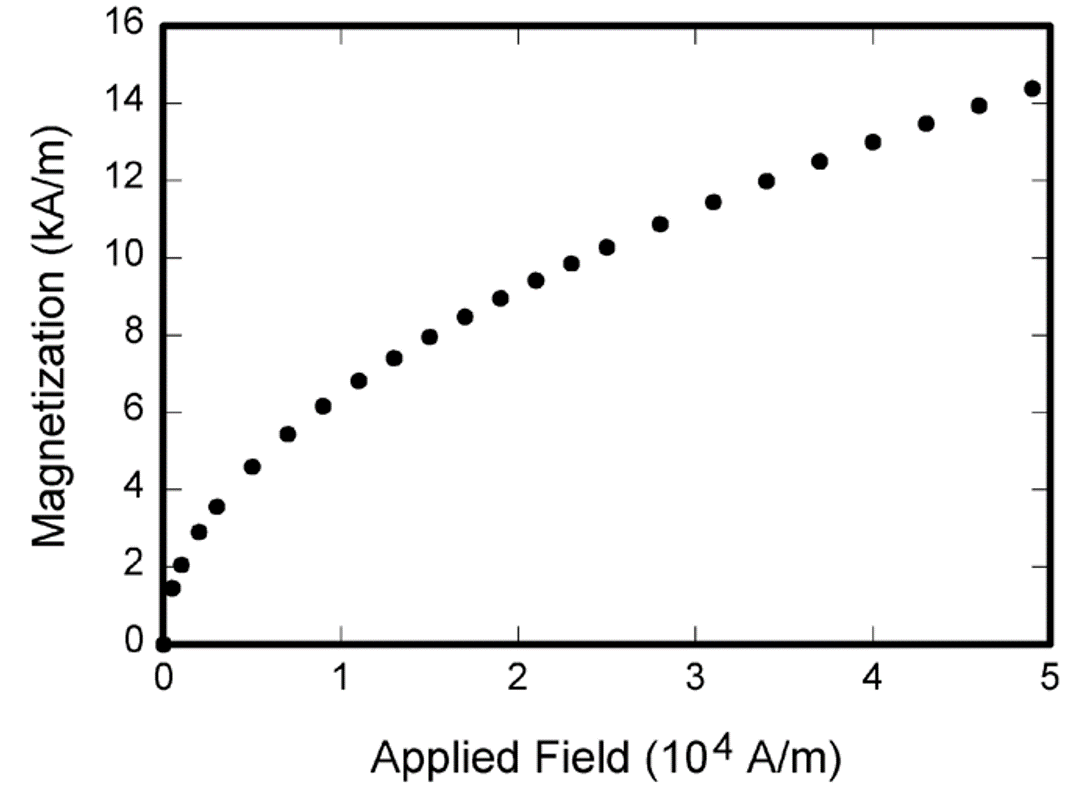
\includegraphics[width=2.5in]{Figure1-template.png}
    \caption{Placeholder for a figure (e.g., AI-Pedia system architecture or pipeline diagram). Replace \texttt{Figure1-template.png} with your own image.}
    \label{fig:my_label}
\end{figure}

% An example of a floating figure using the graphicx package.
% Note that \label must occur AFTER (or within) \caption.
% For figures, \caption should occur after the \includegraphics.
% Note that IEEEtran v1.7 and later has special internal code that
% is designed to preserve the operation of \label within \caption
% even when the captionsoff option is in effect. However, because
% of issues like this, it may be the safest practice to put all your
% \label just after \caption rather than within \caption{}.
%
% Reminder: the "draftcls" or "draftclsnofoot", not "draft", class
% option should be used if it is desired that the figures are to be
% displayed while in draft mode.
%
%\begin{figure}[!h]
%\centering
%\includegraphics[width=2.5in]{myfigure}
%\caption{Simulation results for the network.}
%\label{fig_sim}
%\end{figure}

% An example of a double column floating figure using two subfigures.
% (The subfig.sty package must be loaded for this to work.)
% The subfigure \label commands are set within each subfloat command,
% and the \label for the overall figure must come after \caption.
% \hfil is used as a separator to get equal spacing.
% Watch out that the combined width of all the subfigures on a 
% line do not exceed the text width or a line break will occur.
%
%\begin{figure*}[!t]
%\centering
%\subfloat[Case I]{\includegraphics[width=2.5in]{box}%
%\label{fig_first_case}}
%\hfil
%\subfloat[Case II]{\includegraphics[width=2.5in]{box}%
%\label{fig_second_case}}
%\caption{Simulation results for the network.}
%\label{fig_sim}
%\end{figure*}
%
% Note that often IEEE papers with subfigures do not employ subfigure
% captions (using the optional argument to \subfloat[]), but instead will
% reference/describe all of them (a), (b), etc., within the main caption.
% Be aware that for subfig.sty to generate the (a), (b), etc., subfigure
% labels, the optional argument to \subfloat must be present. If a
% subcaption is not desired, just leave its contents blank,
% e.g., \subfloat[].

\subsection{References}
The list of cited references appears at the end of the report, listed by order of appearance. Citations use individual brackets, e.g. [1], [5]. Citation ranges are formatted as [1], [2], [3], [4] (not [1]-[4]). When citing a section in a book, give the relevant page numbers [2]. At the beginning of a sentence use author names instead of ``Reference [3],'' e.g. ``Smith and Smith [3] show ...''

\section{Methodology}
This section presents the design and implementation of AI-Pedia in detail. The user uploads a ZIP of TXT or PDF documents (minimum 10). The backend extracts keywords (TF-IDF and MMR), queries multiple external sources (Wikipedia, Google Scholar, arXiv, YouTube, GitHub, etc.), cleans and normalises results, runs the CBF recommender (cosine similarity, threshold, AI-keyword filter), optionally generates summaries via an LLM or rule-based fallback, and packages outputs into a downloadable ZIP. The frontend provides upload, progress feedback via server-sent events, and download. Keyword extraction uses TF-IDF vectorisation and MMR for diversity; resource search has separate functions per type (text, video, code) with domain filtering; the recommender builds TF-IDF vectors for user documents and each resource and returns top-$k$ per type. This section should be between 4 to 6 pages in length.

\begin{table}[!h]
% increase table row spacing, adjust to taste
\caption{Main pipeline stages of AI-Pedia}
\label{table_example}
\centering
\renewcommand{\arraystretch}{1.2}
\begin{tabular}{ll}
\hline\hline
Stage & Description\\
\hline
1. Upload & User uploads ZIP of TXT/PDF documents (min.\ 10).\\
2. Keyword extraction & TF-IDF + MMR; output list of queries.\\
3. Multi-source search & Wikipedia, Scholar, arXiv, YouTube, GitHub, etc.\\
4. CBF ranking & Cosine similarity; threshold and AI-keyword filter.\\
5. Summarisation & Optional LLM or rule-based fallback.\\
6. Output & ZIP with \texttt{txt/}, \texttt{video/}, \texttt{code/} folders.\\
\hline\hline
\end{tabular}
\end{table}

% An example of a floating table. Note that, for IEEE style tables, the
% \caption command should come BEFORE the table and, given that table
% captions serve much like titles, are usually capitalized except for words
% such as a, an, and, as, at, but, by, for, in, nor, of, on, or, the, to
% and up, which are usually not capitalized unless they are the first or
% last word of the caption. Table text will default to \footnotesize as
% the IEEE normally uses this smaller font for tables.
% The \label must come after \caption as always.
%
%\begin{table}[!t]
%% increase table row spacing, adjust to taste
%\renewcommand{\arraystretch}{1.3}
% if using array.sty, it might be a good idea to tweak the value of
% \extrarowheight as needed to properly center the text within the cells
%\caption{An Example of a Table}
%\label{table_example}
%\centering
%% Some packages, such as MDW tools, offer better commands for making tables
%% than the plain LaTeX2e tabular which is used here.
%\begin{tabular}{|c||c|}
%\hline
%One & Two\\
%\hline
%Three & Four\\
%\hline
%\end{tabular}
%\end{table}

\noindent \textit{The pipeline is modular; each stage can be configured or extended independently.}

\section{Results}
This section presents the outcomes of the implemented system. Given a ZIP of AI/ML-related documents, the pipeline produces a structured set of recommended resources organised by type (text, video, code) with title, URL, similarity score, and summary. The ZIP download contains folders \texttt{txt/}, \texttt{video/}, \texttt{code/} with cleaned content or link lists. Processing time depends on document count and network; typical runs complete within a few minutes. Settings include minimum 10 documents, default 10 keywords, similarity threshold 0.05, top-5 per type, and optional OpenAI API for summaries. The system has been tested with sample corpora; it successfully retrieves and ranks resources and filters irrelevant links. Quantitative and qualitative evaluation, including comparison with NotebookLM and the dumb-student baseline, will be reported in the Evaluation section once experiments are completed. This section should be around 2 pages in length.

\section{Evaluation}
This section is reserved for the evaluation and should be between 1 to 2 pages in length. It will include: (1) objective comparison with NotebookLM (same input and tasks; quality rubrics and response time/resource usage); (2) a ``dumb student'' baseline (deliberately limited model vs.\ full pipeline; score deltas and preferences); (3) subjective user questionnaires (e.g., Likert scales on learning benefit, ease of use, trust, and preference). Results, tables, and figures will be added here in a future revision.

\section{Conclusion}
This paper presented AI-Pedia, an AI-powered multimedia resource recommendation system for machine learning education. The system takes user-uploaded documents, extracts keywords with TF-IDF and MMR, searches multiple sources (Wikipedia, Scholar, arXiv, YouTube, GitHub, etc.), and uses content-based filtering to recommend the most relevant text, video, and code resources. Optional LLM summarisation and a rule-based fallback improve the usefulness of each recommendation. The implementation is modular and configurable; a structured evaluation plan has been defined to compare the system with NotebookLM and to quantify the benefit of the full pipeline over a weakened baseline. Future work includes completing the planned evaluation, extending support to more languages and domains, and exploring tighter LLM integration. This section should be no more than 1 page in length. The page lengths given for each section are indicative and will vary from project to project but should not exceed the upper limit. A summary is shown in Table \ref{table_2}.

\begin{table}[!t]
\renewcommand{\arraystretch}{1.3}
\caption{Summary of Page Lengths for Sections}
\label{table_2}
\centering
\begin{tabular}{cc}
\hline\hline
Section & Number of Pages\\
\hline
I. Introduction & 2\\
II. Related Work & 2-3\\
III. Methodology & 4-6\\
IV. Results & 2\\
V. Evaluation & 1-2\\
VI. Conclusion & 1\\
\hline\hline
\end{tabular}
\end{table}


% trigger a \newpage just before the given reference
% number - used to balance the columns on the last page
% adjust value as needed - may need to be readjusted if
% the document is modified later
%\IEEEtriggeratref{8}
% The "triggered" command can be changed if desired:
%\IEEEtriggercmd{\enlargethispage{-5in}}

% references section

% can use a bibliography generated by BibTeX as a .bbl file
% BibTeX documentation can be easily obtained at:
% http://mirror.ctan.org/biblio/bibtex/contrib/doc/
% The IEEEtran BibTeX style support page is at:
% http://www.michaelshell.org/tex/ieeetran/bibtex/
%\bibliographystyle{IEEEtran}
% argument is your BibTeX string definitions and bibliography database(s)
%\bibliography{IEEEabrv,../bib/paper}
%
% <OR> manually copy in the resultant .bbl file
% set second argument of \begin to the number of references
% (used to reserve space for the reference number labels box)

\newpage
\begin{thebibliography}{1}

\bibitem{IEEEhowto:bridle}
J.S. Bridle, \emph{Probabilistic Interpretation of Feedforward Classification Network Outputs, with Relationships to Statistical Pattern Recognition}, Neurocomputing—Algorithms, Architectures and Applications, F. Fogelman-Soulie and J. Herault, eds., NATO ASI Series F68, Berlin: Springer-Verlag, pp. 227-236, 1989. (Book style with paper title and editor)

\bibitem{IEEEhowto:chen}
W.-K. Chen, \emph{Linear Networks and Systems}, Belmont, Calif.: Wadsworth, pp. 123-135, 1993. (Book style)

\bibitem{IEEEhowto:poor}
H. Poor, \emph{A Hypertext History of Multiuser Dimensions}, MUD History, http://www.ccs.neu.edu/home/pb/mud-history.html. 1986. (URL link *include year)

\bibitem{IEEEhowto:elissa}
K. Elissa, \emph{An Overview of Decision Theory}, unpublished. (Unpublished manuscript)

\end{thebibliography}

% that's all folks
\end{document}


